\documentclass[12pt]{article}

\usepackage{helpers}

\begin{document}

Name: \makebox[3in]{\hrulefill
%NAME
\hrulefill}

\vfill

\begin{center}
{\huge Retest 1}

{\large April 11, 2025}
\end{center}

\testrules

\vfill

\pledge

\newpage

%BEGIN_STANDARD_DR

\section*{Data Representation}

Demonstrate understanding of numeric and non-numeric data through conversions and operations on such data. Please show your work!

\begin{enumerate}
\item Convert the (unsigned) binary integer 0b00101101 to decimal.
\vfill

\item Convert the two's complement binary integer 0b11110100 to decimal.
\vfill

\item Convert the decimal integer -45 to two's complement binary.
\vfill

\pagebreak

\item Convert the hexadecimal number 0x28 to binary.
\vfill

\item Compute the following subtraction of two's complement binary integers: 0b11101000 - 0b10011111. 
\vfill

\item Write the string ``CS 241'' as a sequence of ASCII values. An ASCII table is included at the end of this test.
\vfill
\end{enumerate}

\vfill

\standardsfooter

\newpage

%END_STANDARD_DR

%BEGIN_STANDARD_LR

\section*{Logic Representation}

Demonstrate understanding of boolean expressions and operations, logic circuits through computation and modeling.

\begin{enumerate}
\item Consider the boolean function $f(A,B) = (A\textrm{ and }B)\textrm{ OR }(A\textrm{ xor }B)$. Make a truth table for this function.
\vfill

\item The function $f$ above is equivalent to a basic boolean function. Which boolean function is it equivalent to?
\vfill

\pagebreak

\item Draw a logic circuit with two 1-bit inputs, $A$ and $B$, and one output, $C$. The output $C$ is 1 if $A$ and $B$ are equal. Otherwise, $C$ is 0.
\vfill

\item Draw a logic circuit with three 1-bit inputs, $A$, $B$, and $C$, representing the bits of a 2-bit binary integer $AB$ and a 1-bit binary integer $C$. There should be three 1-bit outputs, $D$, $E$, and $F$, representing the bits of the result $DEF = AB + C$.
\vfill
\end{enumerate}

\vfill

\standardsfooter

\newpage

%END_STANDARD_LR

%BEGIN_STANDARD_AP

\section*{Assembly Programming}

Demonstrate understanding of assembly programming by writing a program using global variables, local variables, input with \texttt{scanf}, and/or output with \texttt{printf}.

Write an assembly program called \texttt{thumbs.s} that does the following:
\begin{itemize}
\item Ask the user to enter an integer
\item Read input and store it in a global variable named \texttt{num}
\item Ask the user again to enter an integer (you may reuse the same prompt)
\item Read input and store it in a local variable
\item Load both variables and compute their sum
\item Print a response: ``The sum of those numbers is X'' (replacing X with the actual sum)
\end{itemize}

The comments below lay out the general structure of the program. You may write your code between the comments or on another sheet

\newpage 

\textbf{adder.s}

\begin{verbatim}
@ Global constants




@ Global variables




@ main




    @ stack frame setup, one local variable



     
    @ ask the user to enter a number



     
    @ store the response in num1



     
    @ ask the user to enter a number again



     
    @ store the response in num2




    @ load the values and compute their sum




    @ print the response



     
    @ return 0




    @ stack frame teardown




@ Pointers




\end{verbatim}

\vfill

\standardsfooter

\newpage

%END_STANDARD_AP

%BEGIN_STANDARD_HC

\section*{Hardware Components}

Demonstrate understanding of hardware components and their purposes through answering conceptual questions and identifying components.

\begin{enumerate}
\item What are the two main subcomponents of the CPU? What does each of them do?
\vfill
\item What is the role of a register in a computer?
\vfill
\item What is the role of main memory in a computer?
\vfill
\item What is a byte?
\vfill
\item What is a processor's clock cycle time? What is the relationship between clock cycle time and clock rate?
\vfill

\pagebreak

\item Write a detailed description of what happens in the fetch phase of instruction execution in the von Neumann architecture. Which hardware components and/or special registers are involved?
\vfill
\item Write a detailed description of what happens in the decode phase of instruction execution in the von Neumann architecture. Which hardware components and/or special registers are involved?
\vfill
\item Write a detailed description of what happens in the execute phase of instruction execution in the von Neumann architecture. Which hardware components and/or special registers are involved?
\vfill
\item Write a detailed description of what happens in the store phase of instruction execution in the von Neumann architecture. Which hardware components and/or special registers are involved?
\end{enumerate}

\vfill

\standardsfooter

%END_STANDARD_HC

\newpage

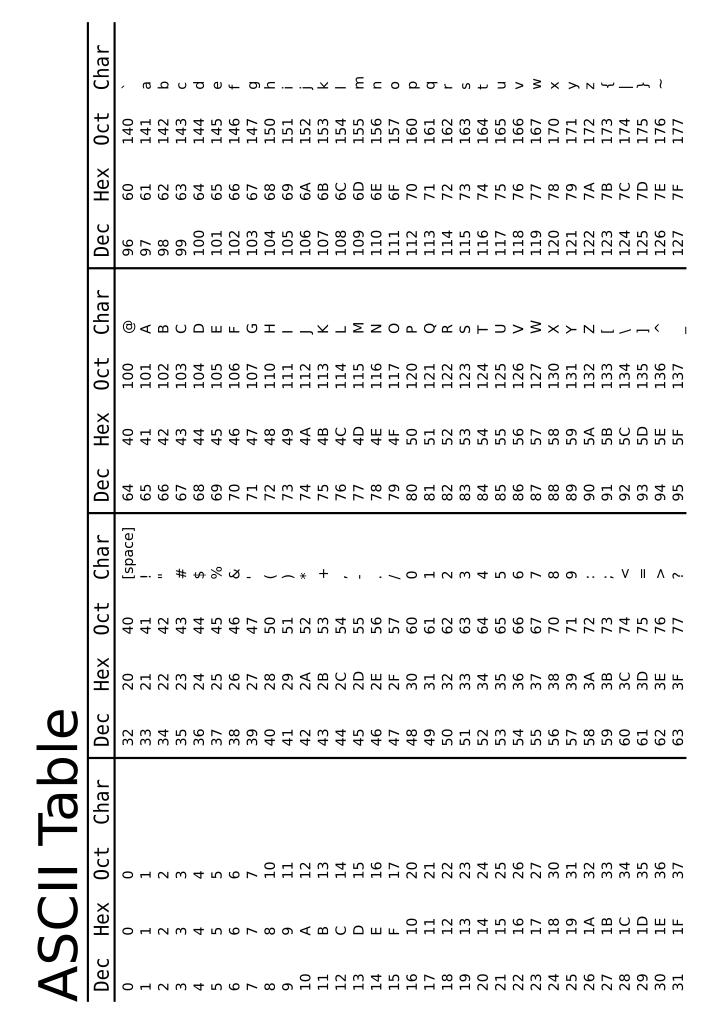
\includegraphics[height=\textheight]{wikimedia-ascii-table.png}

\end{document}